\section {Android application}
\label {Impl_AndroidNodeSection}

	As previously mentioned, the hand terminal uses Android as an operating system and software for it is written mostly in Java and XML. The application was developed in Android Studio(3.0) and uses standard project structure. Project structure can be seen on figure \ref{fig:AndroidProjectStructure}.

\begin{figure}[H]
\centering
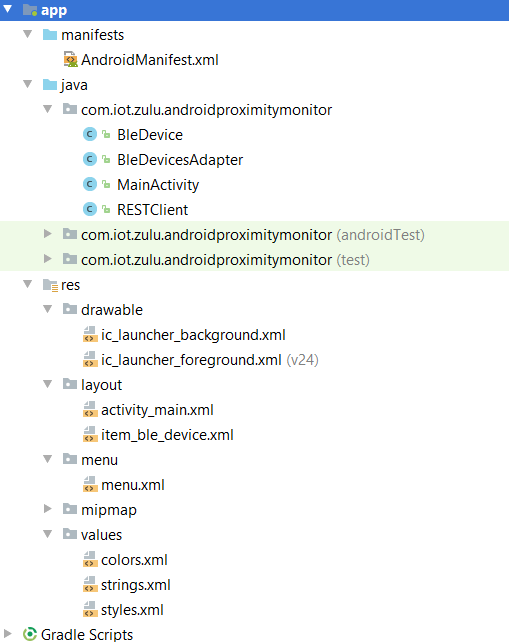
\includegraphics[scale=0.6]{gfx/AndroidProjectStructure}
\caption{Android project structure}~\label{fig:AndroidProjectStructure}
\end{figure}

The application consists of one Activity\cite{Activity}, where nearby BLE devices are displayed on the screen in form of the ListView\cite{ListView}. To properly display all the information about the devices additional Java classes and layout files representing them had to be created along with custom ListView adapter. Final layout of the app is shown on figure \ref{fig:AndroidScreenshots}. First view from the left shows device screen with running application displaying found BLE devices sorted by RSSI. Green highlight of the list element indicates "OK" status of the node. If an element in the list is highlighted in red(as shown in the middle of figure \ref{fig:AndroidScreenshots}) it means that there an alarm raised by that specific node. The technician can tap on this element and a Dialog\cite{Dialog} will appear to display the alarm and resolution information. The data used to build this dialog is retrieved from the central server's database through REST API, specifically calling GET "alarmInfo" method and passing the alarm code in the headers. The dialog allows user to resolve the problem by tapping "Resolve Problem" button. In this case REST PUT "alarmResolution" method will be called.

\begin{figure}[H]
\centering
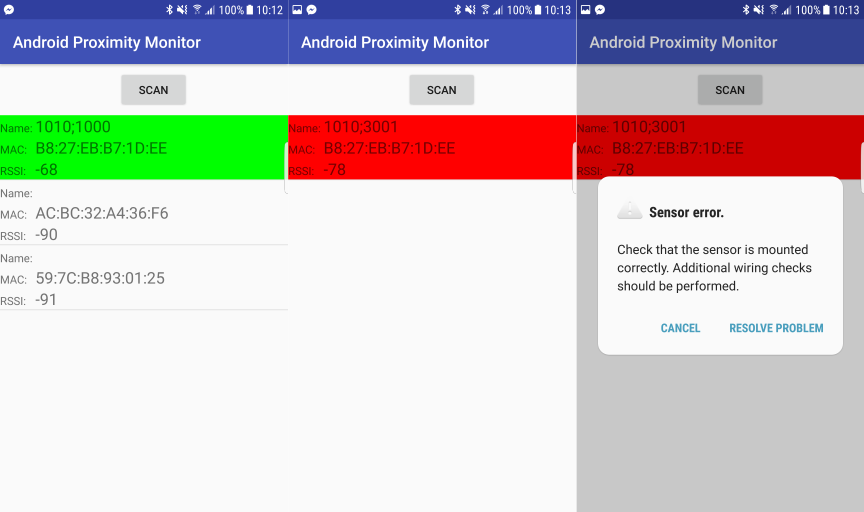
\includegraphics[scale=0.65]{gfx/AndroidScreenshots}
\caption{Android application layout}~\label{fig:AndroidScreenshots}
\end{figure}

Complete overview of Java code of Android project in form of Class diagram is shown on figure \ref{fig:AndroidClass}. 

\begin{figure}[H]
\centering
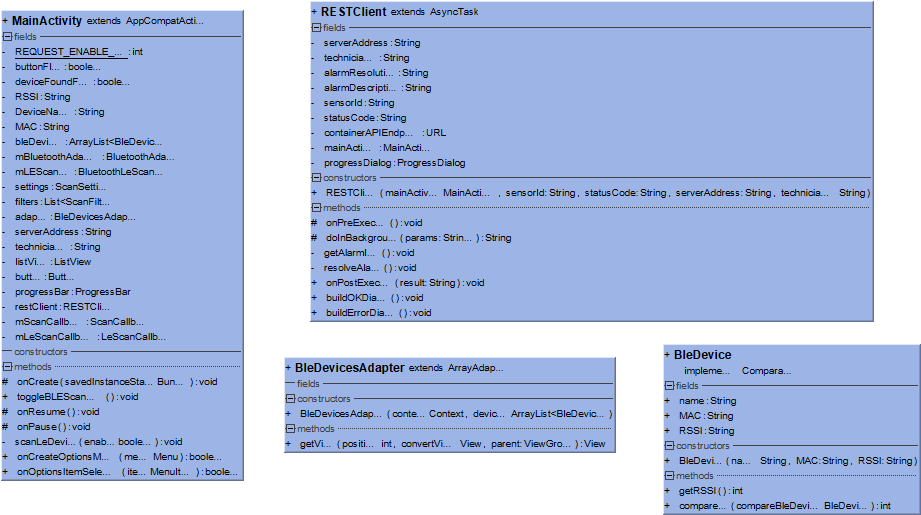
\includegraphics[scale=0.45]{gfx/AndroidClassDiagram}
\caption{Android project class diagram}~\label{fig:AndroidClass}
\end{figure}
